\begin{figure}[h!]
  \centering
    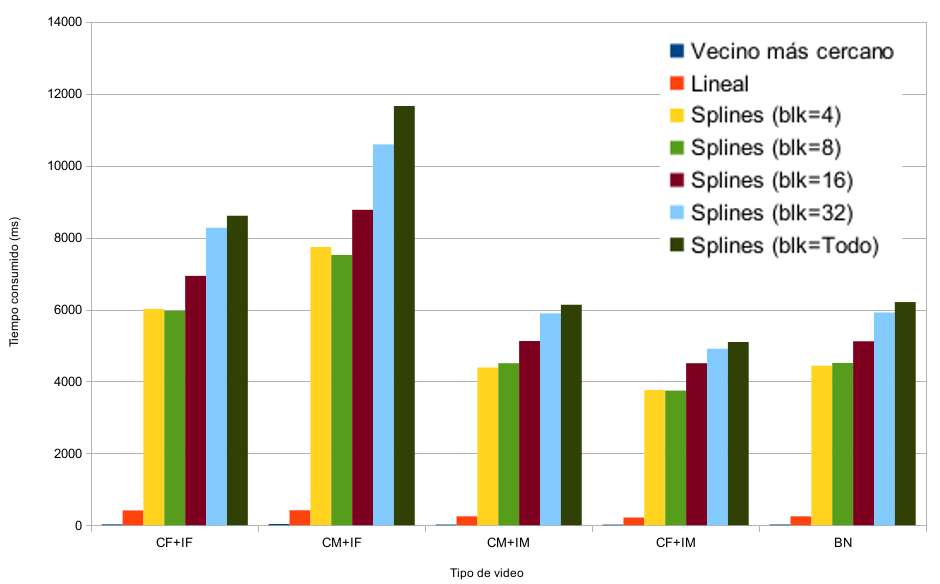
\includegraphics[width=\textwidth]{tiempos-tipo-video.png}
     \caption{Tiempo de ejecución de cada método por tipo de video}\label{fig:tiempos}
\end{figure}
\noindent


\begin{figure}[h!]
  \centering
    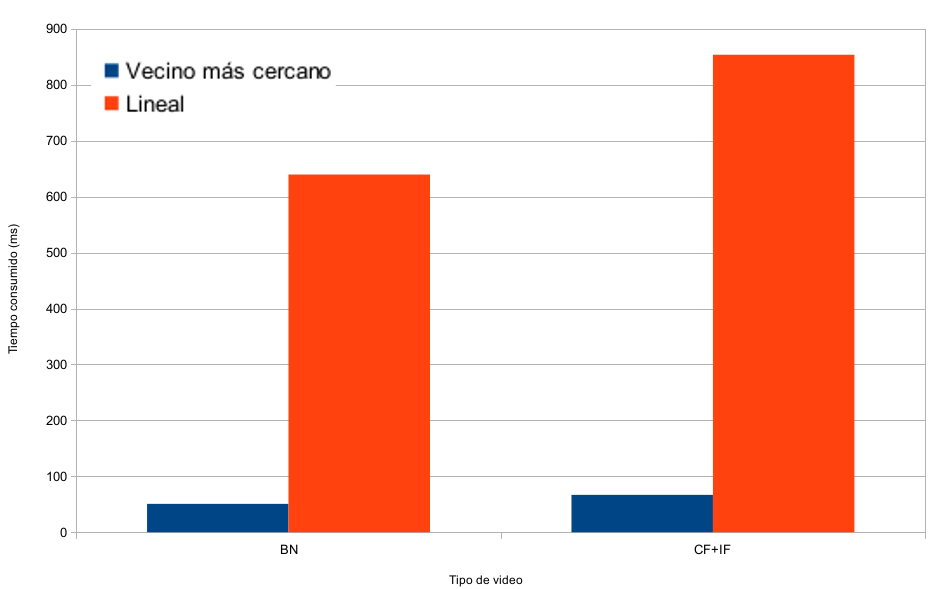
\includegraphics[width=\textwidth]{tiempos-laboratorio.png}
     \caption{Tiempo de ejecución de cada método por tipo de video, para videos de ``laboratorio''}\label{fig:tiempos-lab}
\end{figure}
\noindent

\begin{figure}[h!]
  \centering
    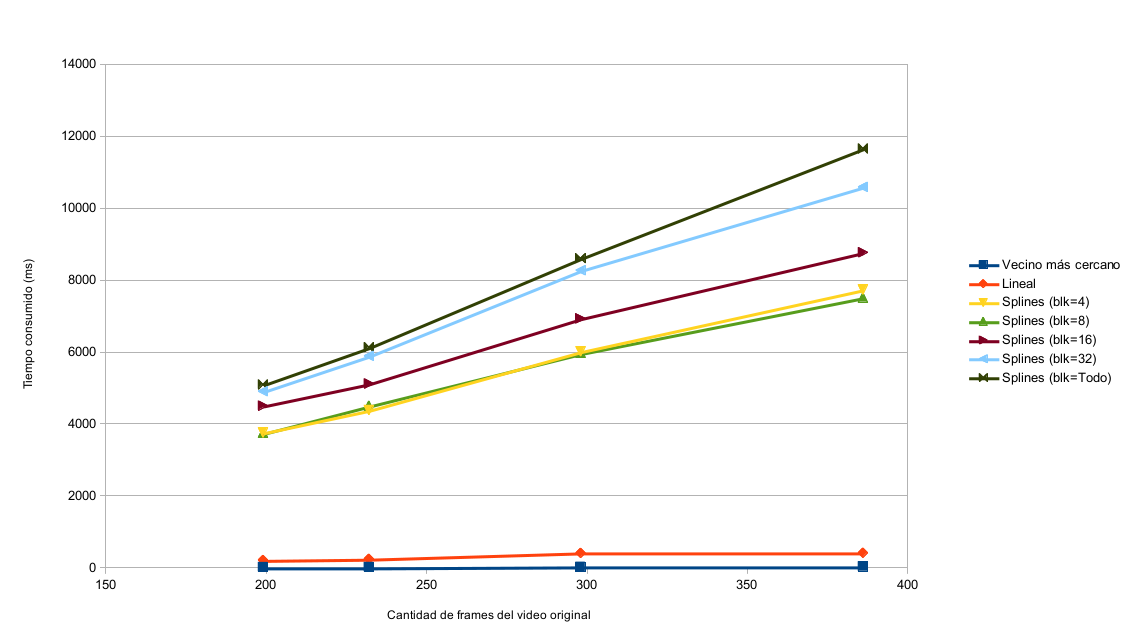
\includegraphics[width=\textwidth]{tiempos-cant-frames.png}
     \caption{Tiempo de ejecución de cada método por cantidad de frames del video}\label{fig:tiempos-cant-frames}
\end{figure}
\noindent


Al medir los tiempos de los métodos para cada tipo de video utilizado, fijando en 10 la cantidad de frames a agregar, obtuvimos lo graficado en la figura \ref{fig:tiempos}. Puede apreciarse claramente, como podía adivinarse, que el método de interpolación por splines tarda mucho más que los demás, mientras que el método de vecino más cercano toma tiempos casi imperceptibles, menores a 30ms para cualquier tipo de video.

Un resultado notable es que, para la interpolación por splines, la relación entre el tamaño de los bloques de frames y el tiempo consumido no resultan proporcionales. Esto puede explicarse con el hecho de que, si bien un tamaño de bloque menor implica que los sistemas de ecuaciones sean menores, también hace que sean más sistemas. Y viceversa: a mayor tamaño de bloque, menos bloques hay y por lo tanto menos sistemas hay que resolver. Según observamos en nuestros experimentos, el tamaño de bloque necesario para obtener la mejor perfomance oscila entre 4 y 8 frames, dependiendo del tipo de video.

De modo similar, observamos que tomar el video completo como un único bloque no es mucho peor que considerar bloques de tamaño 32 frames (al menos no con los videos que utilizamos, de pocos segundos). Asociamos esto al hecho de que, en ese caso, hace falta resolver un único sistema de ecuaciones.

Para los dos métodos más rápidos, realizamos el mismo experimento para nuestros videos de ``laboratorio'': el pasaje de negro a blanco y la foto fija convertida en un video constante. En la figura \ref{fig:tiempos-lab} pueden observarse los resultados, donde nuevamente se confirma que el método de Vecino más cercano es hasta un orden de magnitud más rápido que el de Interpolación lineal.

Finalmente, realizamos la comparación del tiempo consumido por cada método y la cantidad de frames del video original. Los resultados pueden verse en la figura \ref{fig:tiempos-cant-frames}. De su observación notamos que el costo de ejecutar los métodos depende directamente de la cantidad de frames del video, pero que esta dependencia parece ser más fuerte para los splines que para los demás métodos.